\documentclass[11pt,a4paper]{article}
\usepackage[margin=2.6cm]{geometry}
\usepackage[T1]{fontenc}
\usepackage{lmodern}
\usepackage[letterspace=180]{microtype}
\usepackage{booktabs}
\usepackage{amsmath}
\usepackage{parskip}
\usepackage{xcolor}
\usepackage{tikz}
\usetikzlibrary{shapes.geometric,arrows.meta,positioning}
\usepackage[most]{tcolorbox}
\usepackage{titlesec}
\usepackage{caption}
\usepackage{graphicx}

\definecolor{bcnavy}{RGB}{24,38,68}
\definecolor{bcgold}{RGB}{198,160,74}
\definecolor{bcteal}{RGB}{23,110,120}
\definecolor{bcgrey}{RGB}{95,95,95}
\definecolor{bcred}{RGB}{160,60,50}

\titleformat{\section}{\bfseries\large\color{bcnavy}}{\thesection.}{0.6em}{}
\titleformat{\subsection}{\bfseries\color{bcteal}}{}{0em}{}
\captionsetup{font={footnotesize},labelformat=empty,textfont={color=bcgrey}}
\newcommand{\tabnote}[1]{\begin{center}\begin{minipage}{0.92\textwidth}
  \footnotesize\color{bcgrey}#1\end{minipage}\end{center}}

\begin{document}

% ---------------------------------------------------------------- cover
\begin{titlepage}
\centering
\vspace*{3.2cm}

\includegraphics[width=5cm]{bc_logo.pdf}

\vspace{1.6cm}
{\color{bcnavy}\rule{7cm}{0.6pt}}

\vspace{0.9cm}
{\LARGE\bfseries\color{bcnavy} The Evolution of\\[0.15cm] Bayesian Capital\par}
\vspace{0.35cm}
{\large\color{bcnavy} From a thesis about volatility to a nine-name systematic
book:\\ the sequence of decisions, what forced each one,\\ and what the
evidence kept and killed along the way\par}

\vspace{0.9cm}
{\color{bcgold}\rule{7cm}{1.0pt}}

\vspace{1.5cm}
{\bfseries Bayesian Capital}\\[0.2cm]
{\color{bcgrey} Systematic Trading Research}\\[0.9cm]
{\itshape\color{bcgrey} Internal document --- strictly confidential}\\[0.3cm]
{\color{bcgrey} 25 August 2026}
\vfill
\end{titlepage}

% ---------------------------------------------------------------- header
\begin{center}
{\Large\bfseries\color{bcnavy} The Evolution of Bayesian Capital}\\[0.15cm]
{\color{bcnavy} nine stages, each forced by the last}\\[0.25cm]
{\small\color{bcgrey} Bayesian Capital --- Systematic Trading Research
\;$\bullet$\; current book: TSM $\cdot$ VRT $\cdot$ VST $\cdot$ RKLB $\cdot$ MU
$\cdot$ GM $\cdot$ VLO $\cdot$ CF $\cdot$ MRVL}
\end{center}
\vspace{0.1cm}
{\color{bcnavy}\hrule height 0.8pt}
\vspace{0.4cm}

\section{The arc at a glance}

\begin{center}
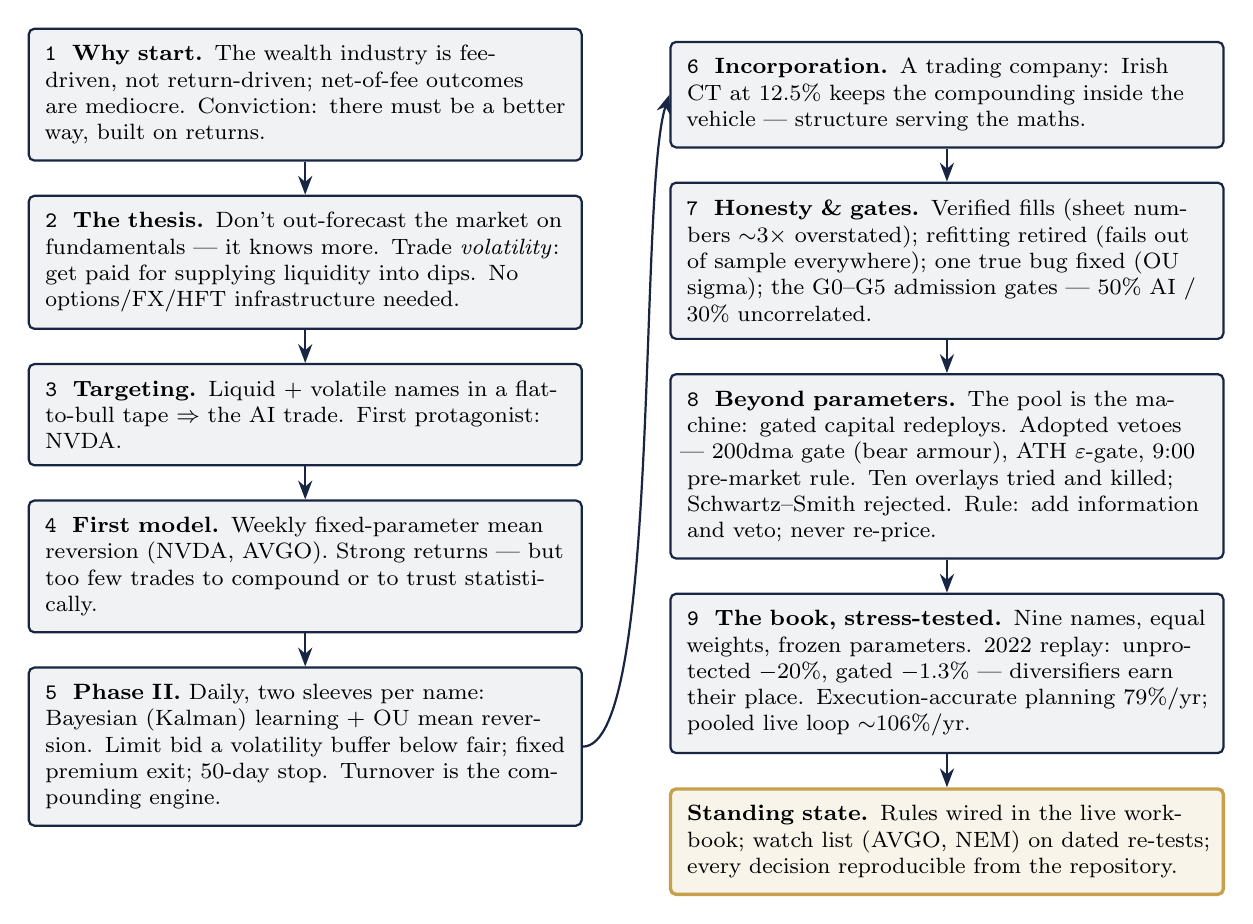
\begin{tikzpicture}[
  st/.style={rectangle, rounded corners=2pt, draw=bcnavy, thick, fill=bcnavy!6,
             text width=6.6cm, align=left, font=\footnotesize, inner sep=6pt},
  tt/.style={font=\footnotesize\bfseries\color{bcnavy}},
  fin/.style={rectangle, rounded corners=2pt, draw=bcgold, very thick, fill=bcgold!12,
              text width=6.6cm, align=left, font=\footnotesize, inner sep=6pt},
  arr/.style={-{Stealth[length=2.4mm]}, thick, bcnavy},
  node distance=0.42cm]

\node[st] (s1) {{\tt 1 } \textbf{Why start.} The wealth industry is fee-driven,
not return-driven; net-of-fee outcomes are mediocre. Conviction: there must be
a better way, built on returns.};
\node[st, below=of s1] (s2) {{\tt 2 } \textbf{The thesis.} Don't out-forecast
the market on fundamentals --- it knows more. Trade \emph{volatility}: get paid
for supplying liquidity into dips. No options/FX/HFT infrastructure needed.};
\node[st, below=of s2] (s3) {{\tt 3 } \textbf{Targeting.} Liquid + volatile
names in a flat-to-bull tape $\Rightarrow$ the AI trade. First protagonist:
NVDA.};
\node[st, below=of s3] (s4) {{\tt 4 } \textbf{First model.} Weekly
fixed-parameter mean reversion (NVDA, AVGO). Strong returns --- but too few
trades to compound or to trust statistically.};
\node[st, below=of s4] (s5) {{\tt 5 } \textbf{Phase II.} Daily, two sleeves per
name: Bayesian (Kalman) learning + OU mean reversion. Limit bid a
volatility buffer below fair; fixed premium exit; 50-day stop. Turnover is the
compounding engine.};
\node[st, right=1.1cm of s1] (s6) {{\tt 6 } \textbf{Incorporation.} A trading
company: Irish CT at 12.5\% keeps the compounding inside the vehicle ---
structure serving the maths.};
\node[st, below=of s6] (s7) {{\tt 7 } \textbf{Honesty \& gates.} Verified fills
(sheet numbers $\sim$3$\times$ overstated); refitting retired (fails out of
sample everywhere); one true bug fixed (OU sigma); the G0--G5 admission gates
--- 50\% AI / 30\% uncorrelated.};
\node[st, below=of s7] (s8) {{\tt 8 } \textbf{Beyond parameters.} The pool is
the machine: gated capital redeploys. Adopted vetoes --- 200dma gate (bear
armour), ATH $\varepsilon$-gate, 9:00 pre-market rule. Ten overlays tried and
killed; Schwartz--Smith rejected. Rule: add information and veto; never
re-price.};
\node[st, below=of s8] (s9) {{\tt 9 } \textbf{The book, stress-tested.} Nine
names, equal weights, frozen parameters. 2022 replay: unprotected $-20\%$,
gated $-1.3\%$ --- diversifiers earn their place. Execution-accurate planning
79\%/yr; pooled live loop $\sim$106\%/yr.};
\node[fin, below=of s9] (s10) {\textbf{Standing state.} Rules wired in the live
workbook; watch list (AVGO, NEM) on dated re-tests; every decision
reproducible from the repository.};

\draw[arr] (s1) -- (s2);
\draw[arr] (s2) -- (s3);
\draw[arr] (s3) -- (s4);
\draw[arr] (s4) -- (s5);
\draw[arr] (s5.east) .. controls +(1.0,0) and +(-0.4,-1.2) .. (s6.west);
\draw[arr] (s6) -- (s7);
\draw[arr] (s7) -- (s8);
\draw[arr] (s8) -- (s9);
\draw[arr] (s9) -- (s10);
\end{tikzpicture}
\end{center}

\section{Why start (and why this way)}

The starting observation was about the industry, not the market: wealth
management as offered to Irish private clients is \textbf{fee-driven rather
than return-driven} --- the providers (the Davys of the world) are compensated
on assets and activity, not outcomes, and net-of-fee results reflect it. The
founding conviction was simply that there must be a better way, and that it
had to be built the other way up: returns first, with the operator's interests
identical to the capital's because they are the same pocket.

That framing did real work later: it is why every subsequent decision was
judged on measured net returns rather than narrative, and why the research
culture became adversarial to its own ideas (\S8).

\section{The thesis: trade volatility, not fundamentals}

Two honest admissions shaped the strategy before a line of code existed.
First, \textbf{the market will always have a better view of fundamentals} than
a private operator --- competing with the sell side and every fund on earnings
calls is a losing game. Second, no high-speed infrastructure for options or FX
was available or wanted. What remains when you subtract forecasting and speed
is \textbf{volatility itself}: prices overshoot intraday, and a patient
resting limit order below fair value gets \emph{paid} for absorbing that
overshoot. The edge is discipline and turnover, not information or latency ---
liquidity provision at retail scale. Everything since has been an elaboration
of that one trade.

\section{Stock targeting: the AI trade}

The thesis needs raw material: names \textbf{liquid enough} that limit orders
fill without moving the price, and \textbf{volatile enough} that the premium
harvested per round trip clears fees comfortably, in a tape that is flat to
rising (a dip-buyer's habitat). In 2024 that pointed one place: the AI
complex, with \textbf{NVDA as the first protagonist} and the semis/AI-infra
names around it. The concentration risk was understood and accepted as the
price of volatility --- managing it became stages 7--9's problem.

\section{First model: weekly mean reversion --- right idea, wrong clock}

The first implementation was a \textbf{weekly fixed-parameter mean-reversion
model} on NVDA and AVGO: a Monday bid clamped below the recent peak, a
premium target, a bounded hold. It made strong returns and taught two lessons.
The productive one: \textbf{the trade count was too low} --- a handful of
round trips a year cannot compound capital or produce statistics you can
trust; the clock had to move to daily. The subtler one, learned later on the
same model: its mean-reversion term never actually bound (0 of 120 weeks) ---
the clamp \emph{was} the model. Simple mechanisms doing all the work while
elaborate terms decorate them became a recurring theme.

\section{Phase II: the daily two-sleeve machine}

The daily redesign is the model that still trades. Each name runs \textbf{two
independent sleeves} estimating fair value differently --- a \textbf{Bayesian
Kalman filter} (a learning trend-follower: hidden level and slope, noises
scaled by the day's range) and an \textbf{OU mean-reverter} (an AR(1) pull
toward a rolling mean). Both wrap the same execution policy: rest a limit bid
a volatility buffer ($k\sigma$) below fair, exit at a fixed premium over the
previous close, 50-calendar-day stop. The sleeves disagree constantly (about
half their entry days differ), which is the point --- but at the trade level
both buy dips and sell bounces quickly. \textbf{Turnover is the compounding
engine}: hundreds of verified fills a year at a few percent each, recycled.

\section{Incorporation: structure serving the maths}

Compounding at this cadence is a tax problem before it is anything else. A
trading company under \textbf{Irish corporation tax at 12.5\%} retains
87.5~cents of every realised euro for redeployment, against roughly half that
retention under personal rates --- over years of compounding, the difference
is not marginal, it is the difference between the strategy working and not.
Incorporation (with trading badges and IBKR execution) made the vehicle match
the strategy: realised gains stay in the pot, the pot stays in the market.

\section{Honesty and gates: the research discipline}

Scaling from two names to a book forced the question every backtest faces:
\emph{which of these numbers are real?} Three answers now define the practice.

\textbf{Verified fills.} The workbook books a same-day round trip whenever the
day's low touched the bid and the high touched the target --- daily bars cannot
order those events. Five-minute data proved the sheet numbers were
$\sim$\textbf{3$\times$ overstated}; every figure since is a verified fill
(low provably before high) or it is not counted.

\textbf{Refitting retired.} Parameter re-optimisation beat frozen parameters
in 1 of 18 weekly folds, 6 of 40 daily folds, and lost every fresh-protocol
comparison; likelihood tests found the price process homogeneous. The
standing law: \emph{structural changes can survive; parameter searches do
not.} One genuine bug was fixed along the way (the OU buffer's sigma measured
the trend, not the noise; corrected to AR(1) residuals, worth +7--13pp) ---
the exception that proves the rule, a specification error rather than a fit.

\textbf{Admission gates.} Stock choice was codified as G0--G5: data \&
verifiability; classification by AI-factor beta ($>$0.20 $\Rightarrow$ the
\textbf{50\%} planning gate, uncorrelated names \textbf{30\%}); the frozen
half-sample split; the both-halves rule for structural claims; and the
marginal book test --- a name must out-earn or de-risk the book it joins.
The gates admitted GM, VLO, CF, then MRVL; they declined NVDA, TSLA, AVGO,
AMD, SMCI, CEG, and a diversifier round (FCX, NEM, UAL, LEN) in its entirety
--- the structural finding there being that names volatile enough to pay the
premium are AI-correlated in this era, which raises the value of the three
diversifier seats already held.

\section{Beyond parameters: the pool, the vetoes, and the graveyard}

With parameters frozen and the book chosen, the remaining degrees of freedom
were \emph{capital routing}. The live workbook's allocation loop pools each
morning's cash across the free sleeves --- so a sleeve that stands down does
not idle, it thickens every other order. That mechanism turned out to be where
improvements live. Three vetoes were adopted, each adding information the
model cannot see and each measured on the standard protocol:

\begin{itemize}
\item \textbf{The 200dma gate}: no new bids in a name whose close sits below
its 200-day average. In the replayed 2022 bear it turns $-20\%$ into
$-1.3\%$; in the pooled bull loop it is free. Bear armour.
\item \textbf{The ATH $\varepsilon$-gate}: no order may construct a trade
whose exit needs a print above the all-time high. Free; removes a real trap.
\item \textbf{The 9:00 pre-market rule}: no order whose buy price sits more
than 4\% below the pre-market print --- such orders fill one day in
twenty and fill badly. The first overlay in eleven attempts to improve both
halves: $\sim$10pp of book-level return.
\end{itemize}

Behind those three stands the graveyard that gives them credibility: HAR
realised-volatility sigma (better forecasts, worse trading), a
volatility-regime gate (the book \emph{earns} from stress), vol-scaled
premiums (the fixed premium is a turnover engine), per-stock price stops
(they cut the trades the bull rescues), the circuit breaker as bear armour
(right trigger, weak action), a midday re-pool (afternoon capital can only
chase fallers), fill-probability weighting (equal weights stand), and
Schwartz--Smith as a third sleeve or OU replacement (all fair-value sleeves
correlate $\sim$0.85 --- a third estimator is dilution). The meta-lesson,
earned ten times: \textbf{overlays that reshape the harvest die; overlays
that add information and only veto have a chance --- and a veto may cancel an
order, never re-price it.}

\section{The book, stress-tested and correctly accounted}

The standing configuration: \textbf{nine names, two sleeves each, equal
weights, parameters frozen at admission}, the three vetoes wired into the
live workbook alongside a discretionary carve-out and a manually-updated
discretionary log. Two final pieces of evidence complete the picture.

\textbf{The bear test.} User-supplied 2021--23 five-minute data allowed the
deployed book to be replayed through a real bear market on verified fills.
Unprotected, 2022 costs $-20\%$ (survivable --- no worse than April 2025);
with the 200dma gate, $-1.3\%$, because the pool rotates gated AI capital
into the diversifiers --- \textbf{GM, VLO and CF earn their seats in exactly
the scenario they were admitted for}. The known blind spot is the fast crash
(a name far above its 200dma can fall 40\% unseen --- April 2025's lesson),
which is the circuit breaker's residual niche.

\textbf{Execution-accurate accounting.} The resting sell is a limit order:
a held position that gaps above its target overnight fills at the open, not
the target. 22\% of held exits did exactly that --- money the live book has
always earned and the research model never counted. Correctly accounted, the
book's planning figure is \textbf{$\approx$79\%/yr} (sheet convention 65\%)
and the pooled live loop with all rules measures $\approx$\textbf{106\%/yr}
full-sample ($\approx$142\%/yr on the tested half) at unchanged drawdown.

\begin{tcolorbox}[colback=bcgold!8, colframe=bcgold, boxrule=0.8pt,
  title={\bfseries The thought process, compressed}, coltitle=bcnavy]
Trade the thing you can be paid for (volatility), in the names that carry it
(the AI trade), on the clock that compounds (daily), inside the structure
that keeps the compounding (12.5\% CT), measured on the only basis that is
real (verified fills), improved only where evidence survives both halves
(vetoes, not re-fits), and stress-tested against the regime that hasn't
happened yet (2022 replay). Each stage was forced by the failure mode of the
one before it.
\end{tcolorbox}

\vspace{0.4cm}
{\color{bcnavy}\hrule height 0.8pt}
\vspace{0.2cm}
{\footnotesize\color{bcgrey} Companion documents: \emph{Verified Book Ranking}
(9--19 Aug); \emph{Book Admission Gates} (10--14 Aug); \emph{Three Volatility
Overlays, Tested and Rejected} (14 Aug); \emph{Bear-Market Protection for the
Nine-Name Book} (15--19 Aug); \emph{The Pre-Market Rule} (18 Aug). Every
figure herein is reproducible from \texttt{premarket\_study/}; findings
indexed in HANDOVER \S3.}

\end{document}
